% ---------------------------------------------------------------------------------------------------------------
% sec_jellium_cancel.tex  (textbook v2) -- \input inside Section \ref{sec:num-jellium}, after Proposition \ref{prop:ewald}
% Numbers: facts_jellium.md; code: code/jellium_cancel.py; new references: refs_jellium.tex
% ---------------------------------------------------------------------------------------------------------------
\subsection{Where the infinities go: Poisson's equation and a jellium disk}\label{jel:sec}

The proof of Proposition~\ref{prop:ewald} says that the divergent $k=0$ term ``is cancelled exactly by'' the
background. This subsection does the same cancellation by hand, in real space, on a finite disk of particles, so that
you can see each infinite term grow and then disappear in the sum (it answers a reviewer's request on version~1).
Conventions are those of this chapter: unit charges, $e^2=1$, density $n=1$ unless written otherwise, each pair of
particles counted \emph{once}, as in~\eqref{eq:ewald} and in the crate. (The Lean quantity \lean{diskEnergy} counts
ordered pairs, and Chapter~5's $J_{s,R}$ in~\eqref{ch5:eq:jellium} does too; both are twice ours.) `Coulomb' means the
three-dimensional law $1/r$ restricted to the plane (Riesz $s=1$); the planar logarithm (Riesz $s=0$) is treated
briefly at the end.

\begin{warnbox}[: two different infinities]
A system of point charges has \emph{two} kinds of divergence, and they are cured by different means.
\begin{itemize}[leftmargin=*]
\item \emph{Short distance, $i=j$.} The ``energy of a point charge with itself'' is $g(0)=\infty$. It is never
  cancelled by anything. It is \emph{excluded} by definition: the sums run over $i\ne j$. In the Ewald formula the
  term $-N\alpha/\sqrt\pi$ only removes the finite value $\operatorname{erf}(\alpha r)/r\to2\alpha/\sqrt\pi$ that was
  added when the smooth part was summed over all pairs including $i=j$; it is bookkeeping, not a cancellation of
  $g(0)$.
\item \emph{Long distance, many pairs.} For $g=1/r$ at density $n$ there are about $2\pi n r\,dr$ partners at distance
  $r$, so the potential felt by a particle at the centre of a disk of radius $R$ is about
  $\int^R 2\pi n r\cdot r^{-1}\,dr=2\pi nR$, and the pair energy per particle of the whole disk (each pair once)
  grows like $\frac83nR$ (Proposition~\ref{jel:prop:disk}). This is the divergence the background cancels.
\end{itemize}
Note also the signs. The background's energy with itself is \emph{positive} (it is a charge distribution of one sign).
The large \emph{negative} term is the particle--background attraction, and we shall see that it equals minus
\emph{twice} the background self-energy, to leading order.
\end{warnbox}

\subsubsection{The Poisson equation for particles plus background}\label{jel:poisson}

Let $N$ unit charges sit at $x_1,\dots,x_N\in\R^2$ and let a uniform background of density $n$ occupy a region
$D\subset\R^2$. The total charge density in the plane is
\begin{equation}\label{jel:eq:rho}
\rho(x)=\sum_{i=1}^N\delta_{x_i}(x)-n\,\mathbf 1_D(x),\qquad \int_{\R^2}\rho=N-n|D| .
\end{equation}
The system is \emph{neutral} when $N=n|D|$. The potential is $\varphi=g*\rho$, and the question is which differential
equation it satisfies. The answer depends on $s$.

\paragraph{The logarithm, $s=0$: the true two-dimensional Poisson equation.} For $r=|x|>0$ the radial Laplacian is
$\Delta f=f''+f'/r$, and for $f=-\log r$ it gives $1/r^2-1/r^2=0$. The flux of $-\nabla(-\log r)=x/r^2$ through any
circle around the origin is $2\pi r\cdot r^{-1}=2\pi$, so, as distributions,
\begin{equation}\label{jel:eq:poisson0}
-\Delta(-\log|x|)=2\pi\,\delta_0,\qquad\text{hence}\qquad
-\Delta\varphi=2\pi\Bigl(\sum_{i}\delta_{x_i}-n\,\mathbf 1_D\Bigr)\quad\text{in }\R^2 .
\end{equation}
\tierC{} (standard; the divergence-theorem argument is the proof). This is Chapter~5's $\kappa_0=2\pi$.
Integrated over a disk $B_\rho$ (Gauss's law), $-\oint_{\partial B_\rho}\partial_r\varphi=2\pi\bigl(\#\{x_i\in
B_\rho\}-n|B_\rho\cap D|\bigr)$: the field far from a \emph{neutral} system has zero monopole part.

\paragraph{The Coulomb law $1/r$, $s=1$: not the planar Poisson kernel.} For $f=r^{-1}$ in the plane,
\[
\Delta f=f''+\frac{f'}r=\frac2{r^3}-\frac1{r^3}=\frac1{r^3}\ne0\qquad(r>0),
\]
so $1/r$ is \emph{not} harmonic away from the charge in two dimensions, and no equation of the form
$-\Delta_2\varphi=c\rho$ can hold. It is harmonic in \emph{three} dimensions: $-\Delta_3\,|X|^{-1}=4\pi\delta_0$ for
$X\in\R^3$. The physical picture is charges and background living on the sheet $\{z=0\}$ of three-dimensional space:
\begin{equation}\label{jel:eq:poisson1}
-\Delta_3\Phi(x,z)=4\pi\,\rho(x)\,\delta(z)\quad\text{in }\R^3,\qquad \varphi(x)=\Phi(x,0),
\end{equation}
with $\Phi\to0$ at infinity. \tierC{} (derivation below.) This is the $s=1$ case ($\gamma=s-1=0$, $\kappa_1=4\pi$) of the
field extension used by Petrache--Serfaty and upstream (described before Corollary~\ref{ch5:cor:jellium}); for $s=1$ the
weight $|y|^\gamma$ is identically $1$ and the extension is just ordinary three-dimensional electrostatics.

\emph{The same equation inside the plane.} Use the Fourier convention of this chapter,
$\hat f(k)=\int f(x)e^{-\mathrm ik\cdot x}\,dx$ with $k\in\R^2$ an angular wave vector, and transform
\eqref{jel:eq:poisson1} in $x$ only. Away from $z=0$ it becomes $(|k|^2-\partial_z^2)\hat\Phi(k,z)=0$; the solution
that decays as $|z|\to\infty$ and is continuous at $z=0$ is $\hat\Phi(k,z)=c(k)e^{-|k||z|}$. Integrating
\eqref{jel:eq:poisson1} across the sheet gives the jump condition
$-\bigl[\partial_z\hat\Phi\bigr]_{z=0^-}^{z=0^+}=4\pi\hat\rho(k)$, that is $2|k|c(k)=4\pi\hat\rho(k)$. Hence
\begin{equation}\label{jel:eq:frac}
\hat\varphi(k)=\hat\Phi(k,0)=\frac{2\pi}{|k|}\,\hat\rho(k),\qquad\text{equivalently}\qquad
(-\Delta)^{1/2}\varphi=2\pi\rho\quad\text{in }\R^2,
\end{equation}
where $(-\Delta)^{1/2}$ is the operator with Fourier multiplier $|k|$. \tierC{} for this computation; the general
statement that a fractional Laplacian is the Dirichlet-to-Neumann map of an extension problem is due to Caffarelli and
Silvestre~\cite{caffsilv} \tierL. With $\rho=\delta_0$, \eqref{jel:eq:frac} gives $\widehat{1/|x|}(k)=2\pi/|k|$, the
transform used in the proof of Proposition~\ref{prop:ewald} (in upstream's convention
$\hat f(\xi)=\int fe^{-2\pi\mathrm ix\cdot\xi}$ it reads $1/|\xi|$; the operator identity does not depend on the
convention). And $\hat\varphi(k)$ stays bounded as $k\to0$ only if $\hat\rho(0)=\int\rho=0$: the $k=0$ divergence of
Proposition~\ref{prop:ewald} is the Fourier face of non-neutrality. For smooth $\rho$ the energy
$\frac12\int\varphi\rho=\frac1{8\pi}\int_{\R^3}|\nabla\Phi|^2\ge0$ is a positive quadratic form; the renormalized energy
of Petrache--Serfaty is this field energy with the point charges truncated (Chapter~5, \tierL).

\subsubsection{Three terms on a disk}\label{jel:three}

Now take a finite piece of the lattice: $x_1,\dots,x_N$ are the points of $\Lat$ in the closed disk of radius $R$
around a centre $c$, and the background is the disk $D$ of radius $R_b$ around the same centre, with
\begin{equation}\label{jel:eq:Rb}
n\pi R_b^2=N\qquad\text{(exact neutrality; $R_b\approx R$).}
\end{equation}
Expanding $\frac12\iint g(x-y)\rho(x)\rho(y)$ with $\rho$ from~\eqref{jel:eq:rho} and dropping $i=j$ gives
\begin{equation}\label{jel:eq:three}
E=\underbrace{\frac12\sum_{i\ne j}g(x_i-x_j)}_{U_{pp}}
\;\underbrace{-\,n\sum_{i=1}^N\int_Dg(x_i-y)\,dy}_{U_{pb}}
\;+\;\underbrace{\frac{n^2}2\int_D\!\!\int_Dg(x-y)\,dx\,dy}_{U_{bb}} .
\end{equation}
Let $\Phi_D(x)=n\int_Dg(x-y)\,dy$ be the potential of the background (the sign of its charge left out). Then
$U_{pb}=-\sum_i\Phi_D(x_i)$ and $U_{bb}=\frac n2\int_D\Phi_D$.

\begin{proposition}[the uniform disk, $g=1/r$]\label{jel:prop:disk}
Let $D$ be a disk of radius $R$ with uniform density $n$, and $\Phi_D(x)=n\int_D|x-y|^{-1}\,dy$. Then
\begin{enumerate}[label=(\alph*)]
\item at the centre $\Phi_D=2\pi nR$, on the rim $\Phi_D=4nR$, and for $|x|=r\le R$,
  $\Phi_D(x)=4nR\,E(r/R)$, where $E(k)=\int_0^{\pi/2}\sqrt{1-k^2\sin^2\theta}\,d\theta$ is the complete elliptic
  integral of the second kind with modulus $k$;
\item $\displaystyle\int_D\!\int_D\frac{dx\,dy}{|x-y|}=\frac{16\pi}3R^3$, hence
  $\displaystyle U_{bb}=\frac{8\pi}3n^2R^3=\frac{8}{3\sqrt\pi}\,n^{1/2}N^{3/2}$ when $N=n\pi R^2$, and
  $U_{bb}/N=\frac83nR$.
\end{enumerate}
\end{proposition}
\begin{humanproof}
\tierC{} (elementary; checked numerically in \S\ref{jel:num}.)
(a) Put the origin of polar coordinates $(\varrho,\theta)$ at the field point $x$, at distance $r$ from the centre.
The area element is $\varrho\,d\varrho\,d\theta$, and the kernel $1/\varrho$ cancels the Jacobian $\varrho$, so
\[
\Phi_D(x)=n\int_0^{2\pi}\!\!\int_0^{\varrho_{\max}(\theta)}\frac{\varrho\,d\varrho}{\varrho}\,d\theta
=n\int_0^{2\pi}\varrho_{\max}(\theta)\,d\theta ,
\]
the integral of the \emph{distance to the boundary} seen from $x$. The ray from $x$ in direction $\theta$ leaves the
disk at $\varrho_{\max}(\theta)=-r\cos\theta+\sqrt{R^2-r^2\sin^2\theta}$ (solve $|x+\varrho e_\theta|^2=r^2+2r\varrho\cos\theta+\varrho^2=R^2$,
with $\theta$ measured from the radial direction through $x$). The term
$-r\cos\theta$ integrates to zero over a full turn, and the square root is $\pi$-periodic and even, so
\[
\Phi_D(x)=4n\int_0^{\pi/2}\sqrt{R^2-r^2\sin^2\theta}\,d\theta=4nR\,E(r/R).
\]
At $r=0$, $E(0)=\pi/2$ gives $2\pi nR$; at $r=R$, $E(1)=\int_0^{\pi/2}\cos\theta\,d\theta=1$ gives $4nR$. (Directly: seen
from a rim point the disk is $\{\varrho<2R\cos\theta,\ |\theta|<\pi/2\}$ and $\int_{-\pi/2}^{\pi/2}2R\cos\theta\,d\theta=4R$.)

(b) Build the disk from the inside out. When the disk has radius $r$, bring the next ring of charge
$dq=n\,2\pi r\,dr$ in from infinity and lay it on the rim. By (a) the work done is $\Phi_{D_r}(\text{rim})\,dq=4nr\cdot
2\pi nr\,dr$, up to the ring's interaction with itself, which is $O(dr^2\log(1/dr))=o(dr)$ and does not contribute to
the integral. The total work is the self-energy:
\[
U_{bb}=\int_0^R4nr\cdot2\pi nr\,dr=\frac{8\pi}3n^2R^3 .
\]
Since $U_{bb}=\frac{n^2}2\iint|x-y|^{-1}$, the double integral is $\frac{16\pi}3R^3$. With $R=(N/(\pi n))^{1/2}$,
$U_{bb}=\frac{8\pi}{3}n^2\bigl(\frac N{\pi n}\bigr)^{3/2}=\frac8{3\sqrt\pi}n^{1/2}N^{3/2}$, and dividing by $N=n\pi R^2$
gives $\frac83nR$.
\end{humanproof}

\paragraph{The size of each term.} \tierC{} Proposition~\ref{jel:prop:disk} fixes $U_{bb}$ exactly. The other two terms
are compared with it by a quadrature argument.
\begin{itemize}[leftmargin=*]
\item $U_{pb}=-\sum_i\Phi_D(x_i)$ is minus a lattice-point sum of the function $\Phi_D$, one point per unit area. The
  integral it approximates is $n\int_D\Phi_D=2U_{bb}$. So $U_{pb}\approx-2U_{bb}=-\frac{16\pi}3n^2R_b^3$, i.e.
  $U_{pb}/N\approx-\frac{16}3nR_b$.
\item $U_{pp}=\frac12\sum_{i\ne j}|x_i-x_j|^{-1}$ is a lattice sum approximating
  $\frac{n^2}2\iint|x-y|^{-1}=U_{bb}$. So $U_{pp}/N\approx+\frac83nR_b$.
\end{itemize}
Each term per particle grows linearly in $R_b$, i.e.\ like $N^{1/2}$, and each total like $N^{3/2}$. The leading
coefficients add to $\frac83-\frac{16}3+\frac83=0$. What survives is the \emph{error} of the two quadratures, which is
$O(1)$ per particle. The first quadrature turns out to be very accurate (see below), so the finite energy sits almost
entirely in $U_{pp}-U_{bb}$: the difference between the discrete pair sum and its continuum approximation. This is the
real-space meaning of the Ewald $k=0$ cancellation.

\emph{Why the limit should be the Ewald value.} \tierC{} For $s=1$ the interaction between two neutral unit cells
decays like a dipole pair in the plane, $|x|^{-3}$, which is summable in two dimensions
($\int^\infty r\cdot r^{-3}\,dr<\infty$). So, unlike three-dimensional Coulomb sums, there is no shape-dependent
surface term, and the disk limit should equal the torus value $e_{\rm tri}$ of~\eqref{eq:ewald}. We do not prove this;
the numerics test it.

\emph{Edge correction.} \tierC{} The particles near the rim do not see a full neighbourhood, so one expects an excess
energy proportional to the perimeter, $\propto R_b\propto N^{1/2}$ in total, hence $\propto N^{-1/2}$ per particle.
Whether the coefficient is a constant, or carries a slowly varying factor such as $\log N$, is a question we answer
only numerically.

\subsubsection{Numerical check}\label{jel:num}

The script \texttt{code/jellium\_cancel.py} (numpy and scipy; it runs in about 6 seconds on two cores) computes the
three terms of~\eqref{jel:eq:three} for disk patches of $\Lat$ with $6\le R\le200$ (up to $N\approx1.26\times10^5$),
each for six random centres $c$, with exact neutrality~\eqref{jel:eq:Rb}. $U_{pp}$ is exact: the number of pairs with
lattice difference $v$ is the autocorrelation of the patch's indicator, an integer array computed by FFT and rounded.
$U_{pb}$ uses Proposition~\ref{jel:prop:disk}(a), plus the exterior formula
$\Phi_D=4nr[E(R_b/r)-(1-R_b^2/r^2)K(R_b/r)]$ for the few points with $R_b<|x_i-c|\le R$ (5.7 on average at $R=200$);
both are checked against the chord integral of the proof. (Trap: \texttt{scipy.special.ellipe} takes the
\emph{parameter} $m=k^2$, not the modulus.) $U_{bb}$ is Proposition~\ref{jel:prop:disk}(b). The reference $e_{\rm tri}$
is recomputed by a one-cell Ewald sum~\eqref{eq:ewald} in Python. The pass criteria were written into the script before
its first run; the radii $R=300,450$ and the $s=0$ negative controls were added afterwards and are labelled so.

\begin{numbox}[: three divergent terms, one finite sum ($s=1$, Tier X)]
Ingredient checks (all \texttt{PASS}): disk potential closed form vs chord quadrature, max relative error
$1.50\times10^{-15}$; $\iint_{D\times D}|x-y|^{-1}$ on the unit disk by quadrature $16.755160819145566$ against
$16\pi/3=16.755160819145562$; FFT pair sums against brute force (254 points) agree to round-off ($0$ relative error);
Python Ewald $e_{\rm tri}=-1.960515789320$ for $\alpha=1,2,4$, differing from the crate value by $1.1\times10^{-13}$.

Means over six centres, per particle, pairs once, $n=1$:
\begin{center}\footnotesize\setlength{\tabcolsep}{4pt}
\begin{tabular}{@{}rrrrrrrr@{}}
\toprule
$R$ & $N$ & $U_{pp}/N$ & $U_{pb}/N$ & $U_{bb}/N=\frac83R_b$ & $e=E/N$ & $e-e_{\rm tri}$ & $\sqrt N(e-e_{\rm tri})$\\
\midrule
6.00 & 113.2 & 14.095 & $-32.011$ & 16.005 & $-1.911915$ & $4.860\times10^{-2}$ & 0.516\\
23.11 & 1678.0 & 59.683 & $-123.260$ & 61.630 & $-1.947564$ & $1.295\times10^{-2}$ & 0.531\\
89.04 & 24906.0 & 235.479 & $-474.872$ & 237.436 & $-1.957161$ & $3.354\times10^{-3}$ & 0.529\\
200.00 & 125655.5 & 531.357 & $-1066.632$ & 533.316 & $-1.958888$ & $1.628\times10^{-3}$ & 0.577\\
\bottomrule
\end{tabular}
\end{center}
Over all 14 radii, $|U_{pb}+2U_{bb}|/N\le4.4\times10^{-3}$, and $(U_{pp}-U_{bb})/N$ runs from $-1.9098$ ($R=6$) to
$-1.9589$ ($R=200$): the finite part is carried by the particle--particle sum minus its continuum value.

\emph{Positive control} (convergence to the Ewald value): $|e-e_{\rm tri}|$ falls from $4.860\times10^{-2}$ to
$1.628\times10^{-3}$, a factor $29.9$ (criterion: below $0.02$ at $R=200$ and shrinking by more than $3$): \texttt{PASS}.

\emph{Negative control (i), no background:} $e=U_{pp}/N$ grows from $14.095$ to $531.357$; the prediction
$\frac83R_b=533.316$ gives a ratio $0.9963$. \emph{Negative control (ii), background density $0.9n$ on the same disk:}
$E=U_{pp}+0.9\,U_{pb}+0.81\,U_{bb}\approx(1-0.9)^2U_{bb}$, so the excess should be $0.01\cdot\frac83R_b$; measured
$(e-e_{\rm tri})/(0.01\cdot\frac83R_b)=1.0003$ at $R=200$, where $e=3.3743$. Both controls fire as predicted.

\emph{Edge scaling:} the log--log slope of $|e-e_{\rm tri}|$ against $N$ for $R\ge40$ is $-0.500$, and
$\sqrt N(e-e_{\rm tri})$ stays between $0.49$ and $0.63$ for all 14 radii with no visible trend. A fit with
$e_{\rm tri}$ held fixed ($R\ge20$) gives $e-e_{\rm tri}=0.6059\,N^{-1/2}-2.8230\,N^{-1}$ (rms $3.3\times10^{-4}$); adding a
term $N^{-1/2}\log N$ instead gives it the coefficient $0.0144$ and a slightly \emph{larger} rms ($3.6\times10^{-4}$). So
the data show a positive edge correction $\approx0.6\,N^{-1/2}$ per particle and no evidence of a logarithm, over this
range. Two larger radii added after the first run agree: $\sqrt N(e-e_{\rm tri})=0.5571$ at $R=300$ ($N\approx2.83\times10^5$)
and $0.5605$ at $R=450$ ($N\approx6.36\times10^5$, $e-e_{\rm tri}=7.0\times10^{-4}$). A fit that lets the limit float
returns $-1.961077$, wrong in the fourth significant digit: our fits over $R\le200$ do not pin the Madelung energy
beyond three digits, which is why the Ewald sum is the instrument of record.

Source: \texttt{code/jellium\_cancel.py}; every number is in \texttt{facts\_jellium.md} with the command that printed it.
\end{numbox}

\begin{figure}[ht]
\centering
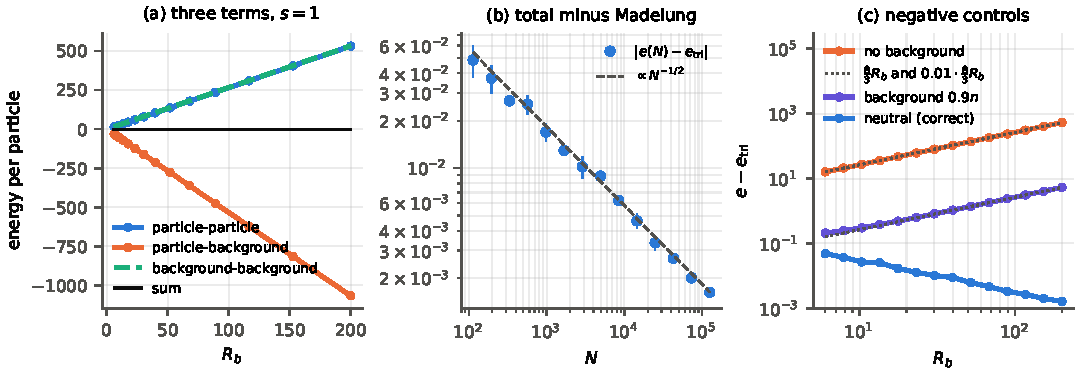
\includegraphics[width=0.9\textwidth]{figures_v2/jellium_cancel.pdf}
\caption{Jellium bookkeeping on triangular-lattice disks, $s=1$, density one, pairs counted once.
(a) The three terms of~\eqref{jel:eq:three} per particle against the background radius $R_b$: particle--particle and
background--background (on top of each other) grow like $+\frac83R_b$, particle--background like $-\frac{16}3R_b$; their
sum (black) is flat at about $-1.96$. (b) Distance of the sum from the Ewald value $e_{\rm tri}=-1.9605157893$, mean and
spread over six disk centres, with an $N^{-1/2}$ guide. (c) Negative controls, $e-e_{\rm tri}$: without background the
energy per particle follows $\frac83R_b$; with background density $0.9n$ it follows $0.01\cdot\frac83R_b$; only the
neutral system converges. \tierX.}\label{jel:fig}
\end{figure}

\paragraph{The logarithm, $s=0$, briefly.} \tierC{} With $g=-\log r$ the same bookkeeping holds with different
growth. By Newton's theorem (from~\eqref{jel:eq:poisson0} and rotational symmetry) the logarithmic potential of the
unit-density disk is $\int_D\log|x-y|\,dy=\pi R^2\log|x|$ outside $D$, and inside it is the radial solution of
$\Delta L=2\pi$ that matches at the rim, $L(r)=\pi\bigl(\frac{r^2}2+R^2\log R-\frac{R^2}2\bigr)$. Integrating over the
disk,
\[
\int_D\!\int_D\log|x-y|\,dx\,dy=\pi^2R^4\Bigl(\log R-\frac14\Bigr),\qquad
U_{bb}=-\frac{N^2}2\Bigl(\log R_b-\frac14\Bigr),
\]
and, by the same quadrature argument, $U_{pp}\approx U_{bb}$ and $U_{pb}\approx-2U_{bb}$. Now each term grows like
$N^2\log N$ (per particle like $N\log N$), not $N^{3/2}$, and again the sum is $O(N)$. Neutrality is not optional here:
adding a constant $c$ to the \emph{kernel} $g$ changes the three terms by $c\frac{N(N-1)}2$, $-cN^2$ and $c\frac{N^2}2$,
which sum to $-\frac c2N$ (not zero, because $i=j$ is excluded); without neutrality the $N^2$ parts would not cancel.
So the value depends on the length unit: $-\log(r/\ell)$ instead of $-\log r$ shifts the energy per particle by
$-\frac12\log\ell$. (An external constant added to the \emph{potential} changes the energy by $c\int\rho=0$; that is a
different statement.) The dipole argument above does not apply to $s=0$, the true planar Coulomb case.

\begin{numbox}[: the logarithm ($s=0$, Tier X)]
A one-cell Ewald sum for $-\log r$ gives $e_{\rm Ewald}=-0.660558714214$ per particle for $\alpha=1,2,4$; there is no
literature value to compare, only $\alpha$-invariance. At $R=200$ the three disk terms per particle are $-317173.03$,
$+634344.74$ and $-317172.37$ ($=-\frac N2(\log R_b-\frac14)$); their sum $-0.657710$ is $2.85\times10^{-3}$ above
$e_{\rm Ewald}$ ($3.75\times10^{-2}$ at $R=6$; positive control \texttt{PASS}). Negative controls: without background
$e=-317173.03$, and with background $0.9n$ the excess is $-3171.72$, both matching the predicted divergent terms to
ratio $1.0000$. The approach is slower and noisier than for $s=1$: the slope for $R\ge40$ is $-0.420$, and
$\sqrt N(e-e_{\rm Ewald})$ wanders between $0.40$ and $1.03$ (six-centre spread up to $8\times10^{-3}$ in $e$). The added
radii give $e-e_{\rm Ewald}=1.51\times10^{-3}$ ($R=300$) and $1.29\times10^{-3}$ ($R=450$), still decreasing. Convergence
to $e_{\rm Ewald}$ is plausible but not established at this precision, and the form of the edge term is undetermined.
\end{numbox}

\subsubsection{What this shows, and what it does not}\label{jel:status}
\begin{itemize}[leftmargin=*]
\item \emph{The rigorous version of this bookkeeping is the Ewald sum.} Proposition~\ref{prop:ewald} organises the same
  cancellation on a torus, where every series converges absolutely and the $k=0$ mode is removed exactly by
  neutrality. The method is Ewald's~\cite{ewald1921} \tierL; the derivation given in this chapter is \tierC.
\item \emph{The disk argument is a heuristic.} The leading-order cancellation $\frac83-\frac{16}3+\frac83=0$ is exact,
  but the claims that the remainder is $O(N)$, that it converges to $e_{\rm tri}$, and that the edge term is
  $\propto N^{-1/2}$ are \tierC{} arguments supported by \tierX{} numerics (Figure~\ref{jel:fig}), not proofs.
\item \emph{The optimality statement is upstream's.} That the triangular lattice minimises the renormalised and jellium
  energies for $0\le s<2$ is Corollary~\ref{ch5:cor:jellium}, proved in upstream's manuscript, \S8~\cite{oai}: \tierL,
  AI-generated, not peer reviewed, and \emph{not formalised in Lean anywhere}. Our numerics computed the energy of
  \emph{one} configuration (the lattice) and compared nothing against competitors.
\item \emph{The cancellation does not bring $s\le2$ under the Lean theorem.} The Lean energy \lean{energy g C} is the
  lower limit of an unsigned sum, in $[0,\infty]$, of an admissible $g\ge0$ over ordered pairs, with no background term.
  Finiteness, \lean{latticeEnergy_riesz_lt_top}, is kernel-checked only for $s>2$; for $s\le2$ the lattice sum
  diverges (\tierC, the counting argument of \S\ref{sec:num-jellium}, not a Lean theorem), so the kernel-checked
  inequality reads $\infty\le\infty$ and says nothing; and $-\log r$ is not admissible at all, since it takes negative
  values. The jellium energy is a different, signed functional obtained by subtracting
  infinities; no Lean statement in this book or upstream is about it.
\end{itemize}

\begin{exercise}\label{jel:ex:frac}
(a) Verify $\Delta_2(r^{-1})=r^{-3}$ for $r>0$ in the plane and $\Delta_3(|X|^{-1})=0$ for $X\ne0$ in space.
(b) Show that the two-dimensional Fourier transform of $|x|^{-1}$ is $2\pi/|k|$ by writing
$|x|^{-1}=\pi^{-1/2}\int_0^\infty e^{-u|x|^2}u^{-1/2}\,du$ and transforming the Gaussians. Compare with~\eqref{jel:eq:frac}.
\end{exercise}

\begin{exercise}\label{jel:ex:riesz}
For $0<s<2$ and $g=r^{-s}$, adapt the proof of Proposition~\ref{jel:prop:disk}: show that the potential of a uniform
disk on its rim is $n\frac{(2R)^{2-s}}{2-s}\int_{-\pi/2}^{\pi/2}\cos^{2-s}\theta\,d\theta$, and that each
of the three terms per particle grows like $R^{2-s}$. What goes wrong at $s=2$? Compare with~\eqref{ch5:eq:locint}.
\end{exercise}

\begin{exercise}\label{jel:ex:mismatch}
Let the background on the disk of~\eqref{jel:eq:Rb} have density $\lambda n$ instead of $n$. Using the quadrature
approximations of \S\ref{jel:three}, show that $E\approx(1-\lambda)^2U_{bb}+O(N)$, so that the energy per particle
diverges like $(1-\lambda)^2\frac83nR_b$ unless $\lambda=1$. Check your formula against negative control (ii) of the
numbox, and run \texttt{code/jellium\_cancel.py} with another value of $\lambda$ (edit the line defining \texttt{e\_09}).
\end{exercise}
